\documentclass{scrartcl}
\usepackage{amsmath}
\usepackage{amssymb}
\usepackage{hyperref}
\usepackage{tikz}
\usepackage{subcaption}
\newcommand{\vol}{\operatorname{vol}}
\begin{document}
Andreas Haupt, Louis Faucon

Topics in Theoretical Computer Science 

Homework IV


\section{Perfect Matchings}\label{sec:perfectmatch}
\begin{enumerate}
\item
It suffices to give a feasible point in the perfect matching polytope of this graph. A theorem by Edmonds proved in class shows, that this polytope is characterized by the inequalities
\begin{align*}
x_e &\ge 0 , \quad \forall e \in E (G) \\
x(\delta (v)) &=1, \quad \forall v \in V(G) \\
x (\delta (S)) &\ge 1, \quad \forall S \subset \binom{V}{k}, k \in 2\mathbb{Z}+1
\end{align*}
We claim, that the point $x$, $x_e = \frac{1}{3}, \forall e \in E(G)$ is feasible. The first $\lvert E(G)\rvert$ inequalities are obviously satisfied, the following $\lvert V(G)\rvert$ by $3$-regularity. For the third consider an odd subset of vertices $S$ of size at least $3$. Clearly, it suffices to show, that $\lvert \delta (S) \rvert \ge 3$. We know
\begin{align*}
\lvert\delta (S)\rvert &\ge 2
\end{align*}
by $2$-connectedness, so it suffices to show, that $\lvert \delta (S) \rvert$ is odd. By a double-counting argument, we have
\begin{align*}
\lvert \delta (S) \rvert + 2\lvert E(G[S])\rvert = 3 \lvert S \rvert
\end{align*}
where the right hand side is odd and the second summand on the left side is even. This shows that $\lvert \delta (S) \rvert$ is odd and completes the proof.
\item
We assign now weights to the edges of graph $G$. We give $f,g$ weight $2$ and the rest weight $1$. Then our (still feasible) solution from the first part has weight
\[
\frac{\lvert V\rvert}{2} + \frac{2}{3}
\]
Now by the integrality of the perfect matching polytope, there is a strictly lighter integral solution. As this one has to have integral weight, it has to be of weight at most $\frac{\lvert V \rvert}{2}$, which means, that there is a perfect matching containing neither $f$ nor $g$.
\item \label{enum:bridge}
Consider such a graph. Let $e=\{v,w\}$ be the unique bridge where $v$ has neighbors $v^1$ and $v^2$ and $w$ has neighbors $w^1$ and $w^2$. Now consider a new graph that has as vertex set
\[
V = (V(G) \setminus \{v,w\})\cup \{v_1, w_1, v_2, w_2\}
\]
and edge set 
\begin{multline*}
E = (E(G) \setminus \{\{v,v^1\},\{v,v^2\},\{w,w^1\},\{w,w^2\}\})\\ \cup \{\{v_1,v^1\},\{v_2,v^2\},\{w_1,w^1\},\{w_2,w^2\},\{v_1,v_2\},\{v_1,w_1\},\{v_2,w_2\},\{w_1,w_2\}\}.
\end{multline*}
This graph then is $3$-regular and $2$-connected as one easily verifies (See Figure \ref{fig:bridge}). By the second part of the task, if we delete edges $\{v_1,v^1\}$ and $\{w_2,w^2\}$, we can find a perfect matching in the graph. This perfect matching has to contain either the edges $\{v_1,w_1\}$ and $\{v_2,w_2\}$ or $\{v_1, v_2\}$ and $\{w_1, w_2\}$. But in both cases, we then get a perfect matching for the original graph by taking the perfect matching in this graph with the exception, that we contract $\{v_1, v_2\}$ and $\{w_1, w_2\}$ calling the vertices resulting from this contraction $v$ resp. $w$ and then including the edge $\{v,w\}$. 

\begin{figure}
\begin{subfigure}[c]{.5\linewidth}
\centering
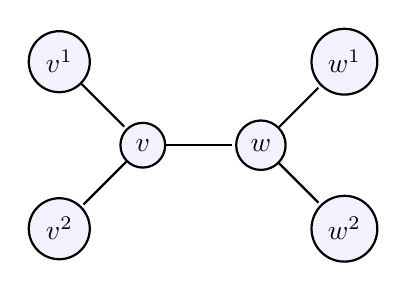
\begin{tikzpicture}[shorten >=1pt,auto,node distance=1.5cm,
  thick,main node/.style={circle,fill=blue!5,draw,}]
  \node[main node] (1) {$v^1$};
  \node[main node] (2)[below right of=1] {$v$};
  \node[main node] (4) [below left of=2] {$v^2$};
  \node[main node] (5) [right of=2] {$w$};
  \node[main node] (7) [above right of=5] {$w^1$};
  \node[main node] (8) [below right of=5] {$w^2$};

  \path[every node/.style={font=\sffamily\small}]
    (1) edge node {} (2)
    (2) edge node {} (5)
        edge node {} (4)
    (5) edge node {} (7)
        edge node {} (8);
   \end{tikzpicture}
   \caption{Original}
   \end{subfigure}
   \begin{subfigure}[c]{.5\linewidth}
   \centering
   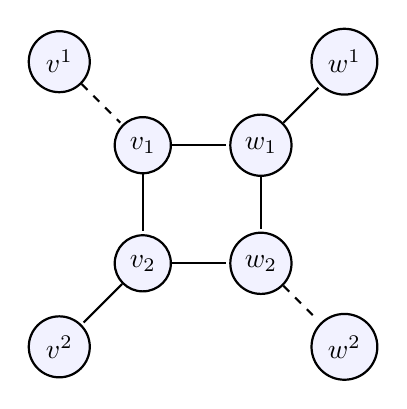
\begin{tikzpicture}[shorten >=1pt,auto,node distance=1.5cm,
  thick,main node/.style={circle,fill=blue!5,draw,}]
  \node[main node] (1) {$v^1$};
  \node[main node] (2) [below right of=1] {$v_1$};
  \node[main node] (3) [below of=2] {$v_2$};
  \node[main node] (4) [below left of=3] {$v^2$};
  \node[main node] (5) [right of=2] {$w_1$};
  \node[main node] (6) [right of=3] {$w_2$};
  \node[main node] (7) [above right of=5] {$w^1$};
  \node[main node] (8) [below right of=6] {$w^2$};
  \path
    (1) edge[dashed] node {} (2)
    (2) edge node {} (3)
        edge node {} (5)
    (3) edge node {} (4)
        edge node {} (6)
    (5) edge node {} (6)
        edge node {} (7)
    (6) edge[dashed] node {} (8);
\end{tikzpicture}
\caption{Dashed will be deleted.}
\end{subfigure}
\caption{Construction made in Task \ref{enum:bridge}.}
\label{fig:bridge}
\end{figure}

\end{enumerate}

\section{Ellipsoid Method}
\begin{enumerate}
\item
An efficient separation oracle for the matrix $A$ is the following:
\begin{itemize}
\item First verify the $m$ inequalities in $O(n^2m)$ time. If it turns out that one of the inequalities is not satisfied, this inequality defines a separating hyperplane that may be returned.

\item Then compute the eigenvectors of the symmetric matrix $A + A^T$ in polynomial time\footnote{This might be done by computing eigenvalues and corresponding eigenvectors of this symmetric matrix using the Jacobi eigenvalue algorithm}. If one of the eigenvectors, $x$, has a negative eigenvalue, a separator hyperplane is $H = \{M\ |\ x^T (M-A) x = 0\}$.
\end{itemize}

Indeed, the second point works because
\[
\forall x\colon  x^T A x = (x^T A x)^T = x^T A^T x
\]

which implies
\[
A \ \text{semidefinite} \iff (A + A^T)\ \text{semidefinite}
\]

and
\[
\forall x\colon x^T (A + A^T) x < 0 \iff x^T A x < 0
\]

\item
First of all, the set of semidefinite matrices is convex and full-dimensional which are good news when we want to apply the Ellipsoid method.

With this efficient separation oracle, we only need for any semidefinite programming polytope $P$
\begin{itemize}
\item an ellipsoid $E_0(P) \supseteq P$
\item a lower bound $B$ on $\vol (K)$ for any full-dimensional semidefinite programming polytope
\item that these two satisfy  $\log(\frac{\vol(E_0(P))}{B})$ polynomial in the input size of $P$
\end{itemize} 
This suffices, as an exponential decrease in volume of the ellipsoids was shown in the lecture:
\[
\vol(E_k)\le e^{-\frac{k}{2(n+1)}} \vol(E_0)
\]
Unfortunately, these two technicalities are not so easily resolved:
\begin{itemize}
\item We cannot use an initial ellipsoid existent for LP, because even though such an initial ellipsoid may be taken if the LP obtained when deleting the semi-definiteness assumption is bounded, but it is not clear to us, why this should always be the case
\item We cannot rely on the LP solution for the minimal polytope stopping criterion because the intersection with the cone of semidefinite matrices can reduce the volume of the polytope. A solution would be only to find an $\epsilon$-approximation of the feasibility problem. Which means we would either give a point of the polytope or conclude it is smaller than a ball of volume $\epsilon$. This phase will require $O(-\log(\epsilon))$ time.
\end{itemize}

\end{enumerate}

\end{document}